\documentclass{beamer}

\usetheme{Warsaw}

\usepackage{amsmath}
\usepackage{apacite}
\usepackage{multimedia}

\author{George G Vega\thanks{\url{mailto:gvegayon@caltech.edu}}}
\institute{Superintendencia de Pensiones}
\title{An\'alisis de Redes}
\date{20 de junio, 2014}

\begin{document}

\frame{\maketitle}

\begin{frame}
\frametitle{Contenidos}
\tableofcontents
\end{frame}

\section{Introducci\'on}

\begin{frame}
\frametitle{Introducci\'on}
\framesubtitle{Objetivos de esta secci\'on}

Esta parte del curso se centrar\'a en lo siguiente:

\begin{itemize}
\item Familiarizarse con el lenguaje
\item Entender gr\'afos desde mirada estad\'istica
\item Realizar an\'alisis de redes utilizando software especializado (Gephi)
\end{itemize}

\end{frame}

\begin{frame}
\frametitle{Introducci\'on}
\framesubtitle{La ciencia de redes}

C\'omo se estudian las redes?

\begin{itemize}
\item {\bf Redes biologicas} Redes de prote\'inas, aliment\'icias, etc.
\item {\bf Redes tecnol\'ogicas} Redes de telecomunicaciones, transporte, etc.
\item {\bf Redes humanas} Amigos, familia, parejas sexuales, etc.
\item {\bf Redes Sociales (virtuales)} Facebook, twitter, etc.
\end{itemize}

En las ciencias sociales es donde se lleva m\'as tiempo desarrollando investigaci\'on
cuantitativa al respecto.

\end{frame}

\section{Definiciones}

\begin{frame}
\frametitle{Definiciones}

\begin{figure}
\centering
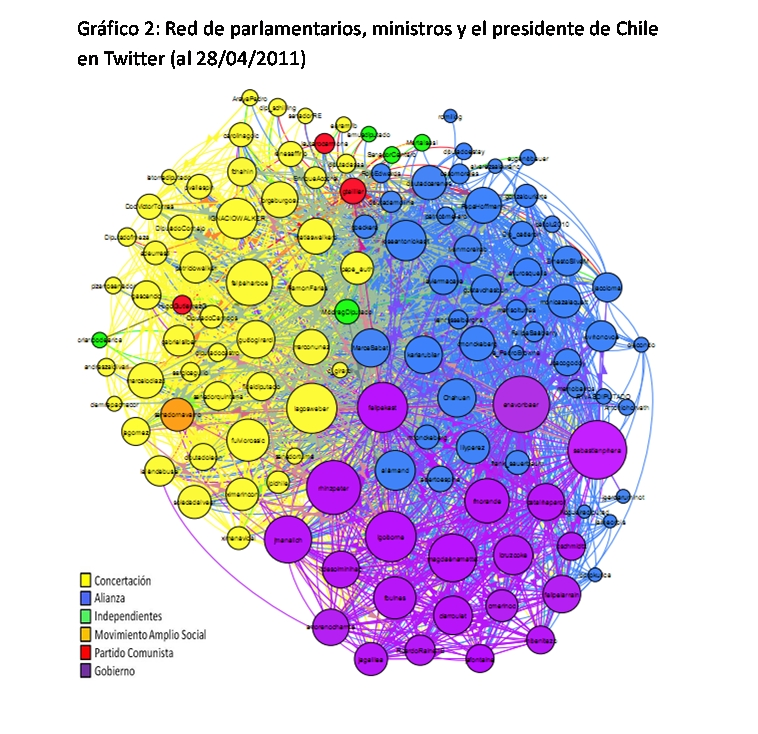
\includegraphics[width=.8\linewidth]{../media/red_parlamentarios_ministros_en_twitter}
\end{figure}
{\footnotesize Fuente: \cite{fabrega2011}}

\end{frame}

\begin{frame}
\frametitle{Definiciones}
\framesubtitle{Conceptos fundamentales}

\begin{itemize}
\item[Vertice] (aka nodo) Unidad fundamental de un grafo.
\item[Conexi\'on] (link) Puede ser dirigida o no.
\item[Grado] (entrada/salida) N\'umero de conexiones de un nodo.
\item[Geod\'esica] Distancia m\'as corta entre dos nodos.
\item[Diametro] Distancia m\'as larga en un g\'rafo. 
\item[Diada] Par de nodos conectados.
\item[Triada] Trio de nodos conectados.
\item[Componente] (gigante) Porci\'on de un grafo desconectado.
\end{itemize}
\end{frame}

\begin{frame}
\frametitle{Definiciones}
\framesubtitle{}

M\'aximo n\'umero de conexiones en un grafo
\begin{equation}
\frac{1}{2}n(n-1)
\end{equation}
\end{frame}

\begin{frame}
\frametitle{Mundos Peque\~nos}

El trabajo de Milgran con sus seis grados de distancia

Se puede medir en funci\'on de la geod\'esica media

\begin{equation}
l = \frac{1}{\frac{1}{2}n(n+1)}\sum_{i\geq j}{d_{ij}}
\end{equation}

Notar que $\frac{1}{2}n(n+1)$ corresponde al m\'aximo n\'umero de links
posibles.
\end{frame}

\section{Estad\'isticos}

\begin{frame}
\begin{itemize}
\item Centralidad de Grado
\item Centralidad de Cercan\'ia
\item Centralidad de Intermediaci\'on
\item Eigen-vector
\item Centralidad
\end{itemize}

Otras medidas de centralidad...
\begin{itemize}
\item N\'umero de Erd{\"o}s \url{}
\item El or\'aculo de Kevin Bacon \url{http://oracleofbacon.org/}
\end{itemize}

\end{frame}

\begin{frame}
\frametitle{Lecturas recomendadas}

\begin{itemize}
\item \cite{newman2003structure}
\item 
\end{itemize}

\end{frame}

\section{Ejemplos}

\begin{frame}
%\movie[options]{placeholder box}{movie filename}
\end{frame}

\section{Referencias}
\nocite{}
\begin{frame}
\frametitle{Referencias}
\bibliographystyle{apacite}
\bibliography{../bib}
\end{frame}


\end{document}

